\input{def}
\begin{document}
\begin{center}
\large{MATH -6890 \hspace{1in} Numerical Solutions of Waves \hspace{1in}Fall 2016\\
Semester Project}\end{center}
Michael Hennessey
\bigskip
\title{A Numerical, Non-Cartesian Grid Euler Equation Godunov Solver}

\begin{abstract}
We describe a method for the numerical solution of the Euler equations for gas dynamics in non-Cartesian geometries. We consider gas flow in two dimensions described by the Euler equations with an ideal equation of state. These equations are solved using a first-order accurate Godunov method for the convective fluxes and a forward Euler time-stepping scheme. We then describe two methods for solving the equations on non-Cartesian domains. Numerical results are presented for each Godunov solver along with numerical convergence results for the numerical solvers, and simulations on square grids and curvilinear grids.
\end{abstract}
\begin{section}{Introduction}
This paper details the creation, stability and accuracy of a first-order conservative numerical solver for the Euler equations on a nonsingular curvilinear grid. We begin by describing first a 1st order Godunov scheme for the 2D Euler equations on a Cartesian grid, an unstructured non-Cartesian grid and on a Curvilinear grid in the following section. In section 3, we compare the exact Riemann solver and the approximate Riemann solver, and demonstrate the proper order of accuracy of the methods which were implemented using both a twilight zone method and a comparison with the exact solution in Section 3. Finally, in Section 4, we will present some simulation results. In Section 5, we will present some concluding remarks and a few directions of further research.
\end{section}
\begin{section}{Methods}
\begin{subsection}{The 1st Order Godunov Scheme on a Cartesian Domain}
We begin by listing the Euler equations
\bq \left[\begin{array}{c}\rho \\ \rho u\\ \rho v \\ E\end{array}\right]_t+\left[\begin{array}{c}\rho u \\ \rho u^2+p \\ \rho u v\\ u(E+p)\end{array}\right]_x+\left[\begin{array}{c}\rho v \\ \rho u v \\ \rho v^2+p \\ v(E+p)\end{array}\right]_y=0,\eq
with ideal gas equation of state $e=\frac{p}{\rho (\gamma-1)}.$
We simplify the above equation by letting
\bq \mbf{u}=\left[\begin{array}{c}\rho \\ \rho u\\ \rho v\\ E\end{array}\right],\;\; \mbf{F(u)}=\left[\begin{array}{c}\rho u \\ \rho u^2+p \\ \rho u v\\ u(E+p)\end{array}\right],\;\; \mbf{G(u)}=\left[\begin{array}{c}\rho v \\ \rho u v \\ \rho v^2+p \\ v(E+p)\end{array}\right].\eq
Thus the Euler equations take the form
\bq \mbf{u}_t+\mbf{F(u)}_x+\mbf{G(u)}_y=0.\eq

We begin by discretizing $\mbf{u}$ to be the cell average defined
\bq \mbf{u}_{j,k}^n=\frac{1}{\dx \dy}\int_{y_{k-1/2}}^{y_{k+1/2}}\int_{x_{j-1/2}}^{x_{j+1/2}}\mbf{u}(\xi,\eta,t_n)d\xi d\eta,\eq
where the $x$ grid is defined to be $x_j=j\dx$ for $j=0,...,M$ and $y$ grid is defined to be $y_k=k\dy$ for $k=0,...,N$ where $\dx=\frac{1}{M}$ and $\dy=\frac{1}{N}$. We then take the cell averages of the solution and the fluxes, and integrate equation (3) in time:
\bq \frac{1}{\dx\dy}\int_{t_n}^{t_{n+1}}\int_{y_{k-1/2}}^{y_{k+1/2}}\int_{x_{j-1/2}}^{x_{j+1/2}}\left[\mbf{u}_t(\xi,\eta,\tau)+\mbf{F}_x(\mbf{u}(\xi,\eta,\tau))+\mbf{G}_y(\mbf{u}(\xi,\eta,\tau))\right]d\xi d\eta d\tau.\eq 
We simplify this equation by integrating out each derivative and rewriting the first two terms:
\bq
\begin{split}
 \mbf{u}_{j,k}^{n+1}-\mbf{u}_{j,k}^n+&\frac{1}{\dx\dy}\int_{t_n}^{t_{n+1}}\int_{y_{k-1/2}}^{y_{k+1/2}}\mbf{F}(\mbf{u}(x_{j+1/2},\eta,\tau))-\mbf{F}(\mbf{u}(x_{j-1/2},\eta,\tau))d\eta d\tau\\
 +&\frac{1}{\dx\dy}\int_{t_n}^{t_{n+1}}\int_{x_{j-1/2}}^{x_{j+1/2}}\mbf{G}(\mbf{u}(\xi,y_{k+1/2},\tau))-\mbf{G}(\mbf{u}(\xi,y_{k-1/2},\tau))d\xi d\tau.
 \end{split}
 \eq
 We now approximate the remaining integrals using the midpoint rule and we get the conservative scheme
\bq \begin{split}
\mbf{u}_{j,k}^{n+1}=\mbf{u}_{j,k}^n-&\frac{\Delta t}{\dx}\left[\mbf{F}(\mbf{u}(x_{j+1/2},y_k,t_{n+1/2}))-\mbf{F}(\mbf{u}(x_{j-1/2},y_k,t_{n+1/2}))\right]\\
-&\frac{\Delta t}{\dy}\left[\mbf{G}(\mbf{u}(x_j,y_{k+1/2},t_{n+1/2}))-\mbf{G}(\mbf{u}(x_j,y_{k-1/2},t_{n+1/2}))\right].
\end{split}\eq
We now need to determine what we mean exactly by the terms $\mbf{u}(x_{j\pm1/2},y_k,t_{n+1/2})$ and $\mbf{u}(x_j,y_{k\pm1/2},t_n).$ In this paper, we will choose to solve the $x$ and $y$ Riemann problems, respectively, to define the terms above using either an exact or approximate solver. This process will be described in the following subsections.\\

The last thing we must discuss as far as discretization is concerned is boundary conditions. We consider only reflective boundaries (as if the gas we are modeling were in an impermeable box) and transmissive boundaries (as if the gas we are modeling were free to move into or out of the domain.\\

In the case of a reflective boundary on the right of the domain, we simply define our ghost cell using the equations
\bq \rho_{M+1,k}^n=\rho_{M,k}^n,\;\; u_{M+1,k}^n=-u_{M,k}^n,\;\;v_{M+1,k}^n=v_{M,k}^n,\;\; p_{M+1,k}^n=p_{M,k}^n.\eq
Clearly, this can be generalized to a reflective boundary on any of the four walls of the domain simply by changing indeces, and moving the negative sign onto the correct normal velocity.\\

For a transmissive boundary, we simply let
\bq \rho_{M+1,k}^n=\rho_{M,k}^n,\;\; u_{M+1,k}^n=u_{M,k}^n,\;\;v_{M+1,k}^n=v_{M,k}^n,\;\; p_{M+1,k}^n=p_{M,k}^n.\eq
This boundary condition can be simply generalized in much the same way as the other boundary condition.
\end{subsection}
\begin{subsection}{Exact Riemann Solver}
We begin with the Riemann problem on the $x$ domain with ideal gas equation of state:
\bq \begin{split}
&\mbf{u}_t+\mbf{F(u)}_x=0,\\
&\mbf{u}(x,y,0)=\left\{\begin{array}{cc}\mbf{u}_L,&x<0,\\ \mbf{u}_R,&x>0\end{array}\right. .
\end{split} \eq
The analysis which creates the exact solver follows from Toro's book, with only the addition of a normal velocity component. We know that our solution to the Riemann problem will consist of a shock or rarefaction wave in the $u-a$ field, a contact discontinuity in the $u$ field, and a shock or rarefaction in the $u+a$ field. This solution is pictured here, with $W$ being a vector of the primitive variables $\rho,u,v,$ and $p$. 
\begin{figure}[h]
\centering
\includegraphics[width=3in]{riemannsoln}
\caption{Wave form of the exact solution to the Riemann problem for the Euler equations}
\end{figure}
We note that we expect the density $\rho$ to jump across shocks and contacts, and smoothly vary over rarefactions, the normal velocity $u$ and pressure $p$ to jump over the shock and change smoothly across the rarefaction waves, and the normal velocity $v$ to jump across the contact discontinuity. This gives rise to the states denoted in the picture of the solution.
\bq W_L=\left[\begin{array}{c}\rho_L\\ u_L\\ v_L\\p_L\end{array}\right],\;\; W_{*L}=\left[\begin{array}{c}\rho_{*L}\\ u_*\\v_L \\p_*\end{array}\right],\;\; W_{*R}=\left[\begin{array}{c}\rho_{*R}\\ u_* \\ v_R\\ p_*\end{array}\right],\;\; W_R=\left[\begin{array}{c}\rho_R \\ u_R\\ v_R\\ p_R\end{array}\right].\eq
Therefore, since we only know the states $W_L$ and $W_R$, we must determine $\rho_{*L},\rho_{*R},u_*,v_*,$ along with the wave types in the 1 and 4 fields and their associated speeds (shock speed, rarefaction tail speeds). We determine these values by parameterizing $\rho_{*R}, \rho_{*L},$ and $u_*$ in terms of $p_*$. We then derive a transcendental equation to solve for $p_*$ using the isentropes across rarefactions and the Rankine-Hugoniot (R-H) conditions across shocks. Next, we will describe an adaptive Newton solver to find the root of this equation, and the wave types in the 1 and 4 fields. Then, the value for $p_*$ found by this Newton solver will be used to find the remainder of the star states, and the shock/rarefaction speeds. Lastly, the full solution will be constructed. \\
\begin{subsubsection}{1 and 4 Shocks}
We begin by assuming that the 1 or 4 wave will be a shock. We first translate into the shock by making the substitution
\bq \hat{u}_1=u_1-S_k,\;\;\; \hat{u}_2=u_2-S_k,\;\;\text{ for }k=L,R.\eq
The R-H conditions are then
\bq \begin{split}
&\rho_1\hat{u}_1=\rho_2\hat{u}_2\\
&\rho_1\hat{u}_1^2+p_1=\rho_2\hat{u}^2+p_2\\
& \rho_1\hat{u}_1v_1=\rho_2\hat{u}_2v_1\\
&\hat{u}_1(\hat{E}_1+p_1)=\hat{u}_2(\hat{E}_2+p_2),
\end{split} \eq
where the 1 state is to the left of the shock, and the 2 state is to the right of the shock. We will generalize this notation later. Clearly, the 3rd condition is the same as the first. We now define the mass flux to be $Q_k\equiv \rho_1\hat{u}_1=\rho_2\hat{u}_2.$ We now substitute this expression into the second R-H condition to get
\bq Q_k\hat{u}_1+p_1=Q_k\hat{u}_2+p_2.\eq
Now, if we reexamine the mass flux definition and set
\bq \hat{u}_1=\frac{Q_k}{\rho_1},\;\;\; \hat{u}_2=\frac{Q_k}{\rho_2},\eq
and substitute these expressions into equation (12) we get
\bq \frac{Q_k^2}{\rho_1}+p_1=\frac{Q_k^2}{\rho_2}+p_2.\eq
We then solve for $Q_k^2$ and see
\bq Q_k^2=\frac{p_2-p_1}{\frac{1}{\rho_1}-\frac{1}{\rho_2}}.\eq
Now we must assume which side of the shock we know the data on. For the sake of this analysis, and without loss of generality we assume we know the 1 state to the left of the shock. We can then solve for $u_2$ in terms of $u_1$ by examining (12) once more by subtracting the kinetic energy terms and moving the pressure terms to the other side:
\bq Q_k(\hat{u}_1-\hat{u}_2)=Q_k(u_1-u_2)=p_2-p_1.\eq
We then have
\bq u_2=u_1-\frac{p_2-p_1}{Q_k},\eq
where $Q_k$ is taken to be the positive root of equation (15) This expression can be simplified as
\bq u_2=u_1-\sqrt{(p_2-p_1)\left(\frac{1}{\rho_1}-\frac{1}{\rho_2}\right)}.\eq
We now investigate the 3rd R-H condition to determine $\rho_2$ in terms of $p_2$, first by rewriting the equation without that hat velocities. We get
\bq \frac{Q_k}{\rho_1}\left[\frac{1}{2}\rho_1\left(\frac{Q_k^2}{\rho_1^2}+v_1^2\right)+\frac{\gamma p_1}{\gamma-1}\right]=\frac{Q_k}{\rho_2}\left[\frac{1}{2}\rho_2\left(\frac{Q_k^2}{\rho_2^2}+v_1^2\right)+\frac{\gamma p_2}{\gamma-1}\right].\eq
Eventually, this simplifies to the relationship
\bq \rho_2=\rho_1\left[\frac{1+\frac{p_2}{p_1}\left(\frac{\gamma+1}{\gamma-1}\right)}{\frac{p_2}{p_1}+\frac{\gamma+1}{\gamma-1}}\right].\eq
We can then use this expression to evaluate $u_2$ solely as a function of the known 1-state variables and $p_2$:
\bq u_2=u_1-(p_2-p_1)\left[\frac{\frac{2}{(\gamma+1)\rho_1}}{p_2+\left(\frac{\gamma-1}{\gamma+1}\right)p_1}\right]^{1/2}.\eq
Now, if we let the 1-state be equivalent to the $L$ state, and the 2-state be equivalent to the $*L$ state, we have exactly the relationship of the variables across the left shock parameterized in terms of $p_*$. However, if we choos the 1-state to be the $*R$ state and the 2-state to be the $R$ state, we must invert the expressions previously derived and solve for the 1-state instead of the 2-state. Fortunately this is fairly simply and can be handled by most symbolic manipulators with ease. To summarize, we get
\bq \rho_{*R}=\rho_R\left[\frac{\frac{p_*}{p_R}+\frac{\gamma-1}{\gamma+1}}{\left(\frac{\gamma-1}{\gamma+1}\right)\frac{p_*}{p_R}+1}\right],\eq
\bq u_*=u_R+(p_*-p_R)\left[\frac{\frac{2}{(\gamma+1)\rho_R}}{p_*+\left(\frac{\gamma-1}{\gamma+1}\right)p_R}\right]^{1/2}.\eq

Then, if we insist that the $u_*$ terms are equivalent, we get a transcendental equation who's root is $p_*$:
\bq (p_*-p_R)\left[\frac{\frac{2}{(\gamma+1)\rho_R}}{p_*+\left(\frac{\gamma-1}{\gamma+1}\right)p_R}\right]^{1/2}+(p_*-p_L)\left[\frac{\frac{2}{(\gamma+1)\rho_L}}{p_*+\left(\frac{\gamma-1}{\gamma+1}\right)p_L}\right]^{1/2}+u_R-u_L=0.\eq
This motivates the definition of the function 
\bq F_k(p)=(p-p_k)\left[\frac{\frac{2}{(\gamma+1)\rho_k}}{p+\left(\frac{\gamma-1}{\gamma+1}\right)p_k}\right]^{1/2},\eq
which we will generalize further in the next subsection. As of now, we leave it at
\bq F_L(p)+F_R(p)+u_R-u_L=0.\eq
\end{subsubsection}
\begin{subsubsection}{1 and 4 Rarefactions}
In the case of a rarefaction wave propagating in the 1 or 4 field, we again seek to parameterize $u_*$, $\rho_{*R}$ and $\rho_{*L}$ in terms of $p_*$. We perform this parameterization by investigating the generalized Riemann invariants
\bq \frac{dp}{d\rho}=a^2,\eq
and
\bq ad\rho+\rho du=0,\eq
where $a$ is the sound speed
\bq a=\sqrt{\frac{\gamma p}{\rho}}.\eq 
The first invariant (27) is then a simple separable equation
\bq \frac{dp}{p}=\gamma\frac{d\rho}{\rho},\eq
which we then integrate from left to right 
\bq \int_{p_1}^{p_2}\frac{dp}{p}=\gamma\int_{\rho_1}^{\rho_2}\frac{d\rho}{\rho}.\eq
This results in the isentropic relationship 
\bq \frac{p_2}{p_1}=\left[\frac{\rho_2}{\rho_1}\right]^\gamma.\eq
Then, as before, we seek to parameterize $\rho$ in terms of $p$, we get
\bq \rho_{*L}=\rho_L\left(\frac{p_*}{p_L}\right)^{\frac{1}{\gamma}},\eq
\bq \rho_{*R}=\rho_R\left(\frac{p_*}{p_R}\right)^{\frac{1}{\gamma}}.\eq
Also from this invariant with $p_2=p$, $\rho_2=\rho$ and $p_1,\rho_1$ undetermined, we can derive the relationship 
\bq p=p_1\left(\frac{\rho}{\rho_1}\right)^\gamma=C\rho^\gamma,\eq
which we will then substitute in to the second invariant (28) to get
\bq \sqrt{\gamma C\frac{\rho^\gamma}{\rho}}d\rho+\rho du=0.\eq
This simplifies considerably to 
\bq \sqrt{\gamma C}\rho^{\frac{\gamma-3}{2}}d\rho=du.\eq
Now, if we integrate from left to right once again, we see
\bq \sqrt{\gamma C}\int_{\rho_1}^{\rho_2}\rho^{\frac{\gamma-3}{2}}d\rho=\int_{u_1}^{u_2}du,\eq
\bq \implies \;\;\frac{2}{\gamma-1}\left(\sqrt{\frac{\gamma C\rho_2^\gamma}{\rho_2}}-\sqrt{\frac{\gamma C\rho_1^\gamma}{\rho_1}}\right)=u_2-u_1.\eq
Then, we can rewrite this using the isentropic relationship (35) as simply
\bq u_2-u_1=\frac{2}{\gamma-1}(a_2-a_1).\eq
Perhaps to be a bit clearer about implementation however, we write the parameterizations for $u_*$ as
\bq u_*=u_L-\frac{2}{\gamma-1}\sqrt{\frac{\gamma p_L}{\rho_L}}\left[\left(\frac{p_*}{p_L}\right)^{\frac{\gamma-1}{2\gamma}}-1\right],\eq
\bq u_*=u_R+\frac{2}{\gamma-1}\sqrt{\frac{\gamma p_R}{\rho_R}}\left[\left(\frac{p_*}{p_R}\right)^{\frac{\gamma-1}{2\gamma}}-1\right].\eq
Then, enforcing that these two parameterizations are equivalent gives us exactly equation (26), although with a different definition of $F$. Therefore, we now expand our definition of $F_k(p)$:
\bq F_k(p)=\left\{\begin{array}{cc}(p-p_k)\left[\frac{\frac{2}{(\gamma+1)\rho_k}}{p+\left(\frac{\gamma-1}{\gamma+1}\right)p_k}\right]^{1/2},&\text{Shock}\\
\frac{2}{\gamma-1}\sqrt{\frac{\gamma p_k}{\rho_k}}\left[\left(\frac{p_*}{p_k}\right)^{\frac{\gamma-1}{2\gamma}}-1\right],&\text{Rarefaction}\end{array}\right. .\eq
We are now poised to find the root of equation (26).
\end{subsubsection}
\begin{subsubsection}{An Adaptive Newton Solver}
We note that although equation (26) does have an exact solution in the case the 1 and 4 waves are both rarefactions, it clearly will not suffice for all Riemann initial data to use a double rarefaction solution. In fact, when solving equation (26), we will not know the wave structure of the solution. Therefore, we cannot even choose a single equation to find the root of. We instead describe the creation of an iterative solver which adaptively chooses which equation to solve based on the relationship between the current iteration's root value and the initial data. This iterative solver takes the form
\bq p^{n+1}=p^n-\frac{F_L(p^n)+F_R(p^n)+u_R-u_L}{F_L'(p^n)+F_R'(p^n)}.\eq
We choose which version of $F_k$ by applying the entropy conditions which state that if $p_k>p^n$ the $k$ wave is a rarefaction and if $p_k<p^n$, we know the $k$ wave is a shock.
\end{subsubsection}
\begin{subsubsection}{The Full Solution of the Riemann Problem}
Now, since the final iteration of our solver will determine the wave-form of our solution, at this point we know the full solution. We need only define a few quantities to generate any solution. The easiest to find are the shock speeds. We use the mass flux defined in equation (15) and substitute it into equation (10) to find $S_k$. This results in the shock speeds
\bq S_L=u_L-a_L\left[\left(\frac{\gamma+1}{2\gamma}\right)\frac{p_*}{p_L}+\frac{\gamma-1}{2\gamma}\right]^{1/2},\eq
\bq S_R=u_R-a_R\left[\left(\frac{\gamma+1}{2\gamma}\right)\frac{p_*}{p_R}+\frac{\gamma-1}{2\gamma}\right]^{1/2}.\eq
Next, we define the head and tail of the rarefaction waves, given respectively by
\bq S_{HL}=u_L-a_L,\;\; S_{TL}=u_*-a_{*L},\eq
on the left, and
\bq S_{HR}=u_R+a_R,\;\; S_{TR}=u_*+a_{*R},\eq
on the right. These quantities bound the rarefaction fans. Finally, we determine the solution inside of the rarefaction waves. The solution of the generalized Riemann invariant (28), along with the characteristic equation
\bq \frac{dx}{dt}=\frac{x}{t}=u-a,\eq
leads to the solution in the fan on the left as
\bq \mbf{u}_{Lfan}=\left\{\begin{array}{c}\rho=\rho_L\left[\frac{2}{\gamma+1}+\frac{\gamma-1}{(\gamma+1)a_L}\left(u_L-\frac{x}{t}\right)\right]^{\frac{2}{\gamma-1}},\\
u=\frac{2}{\gamma+1}\left[a_L+\frac{\gamma-1}{2}u_L+\frac{x}{t}\right],\\
p=p_L\left[\frac{2}{\gamma+1}+\frac{\gamma-1}{(\gamma+1)a_L}\left(u_L-\frac{x}{t}\right)\right]^{\frac{2\gamma}{\gamma-1}}\end{array}\right..\eq
Similarly, solving the invariant (28) along with the characteristic equation on the right wave
\bq \frac{dx}{dt}=\frac{x}{t}=u+a,\eq
results in the solution
\bq \mbf{u}_{Rfan}=\left\{\begin{array}{c}\rho=\rho_R\left[\frac{2}{\gamma+1}-\frac{\gamma-1}{(\gamma+1)a_R}\left(u_R-\frac{x}{t}\right)\right]^{\frac{2}{\gamma-1}},\\
u=\frac{2}{\gamma+1}\left[-a_R+\frac{\gamma-1}{2}u_R+\frac{x}{t}\right],\\
p=p_R\left[\frac{2}{\gamma+1}-\frac{\gamma-1}{(\gamma+1)a_R}\left(u_R-\frac{x}{t}\right)\right]^{\frac{2\gamma}{\gamma-1}}\end{array}\right..\eq
Now all of these quantities have been defined, we can construct the solution for any wave-form. This is achieved by defining the variable $\xi=x/t$, and given the wave-form, we can define any solution. This process is perhaps best described simply by looking through the code attached in the appendix.\\

The last thing we must mention is that in solving the Riemann problem at cell interfaces, we follow the procedure as above, but we simply take $\xi=0.$ Therefore, we can write
\bq \mbf{F}(\mbf{u}(x_{j+1/2},y_k,t_{n+1/2}))=\mbf{F}(\mbf{u}_{j+1/2,k}^{n+1/2}(0)),\eq
where $\mbf{u}_{j+1/2,k}^{n+1/2}(0)$ is the exact solution of the Riemann problem.


\end{subsubsection}

\end{subsection}

\begin{subsection}{Approximate Riemann Solver - HLLC}
An alternative method of calculating the Godunov flux is the Harten, Lax and Van Leer + Contact (HLLC) approximate solver from Toro, Spruce and Speares (1992). This solver is an adaptation of the original HLL solver, which assumes a two-wave configuration. The HLL solver is correct, then, only for hyperbolic systems of two equations. As a consequence, physical features like contact surfaces can have very poor resolution. The HLLC solver presents a three-wave model solution with two star states.\\
\begin{figure}[ht]
\centering
\includegraphics[width=3in]{hllcSoln}
\caption{HLLC approximate Riemann solver}
\end{figure}

To construct the HLLC solver, we inspect again the Riemann problem
\bq \begin{split}
&\mbf{u}_t+\mbf{F}_x+\mbf{G}_y=0,\\
&\mbf{u}(x,y,0)=\left\{\begin{array}{cc}\mbf{u}_L,&x<0\\ \mbf{u}_R,&x>0.\end{array}\right.\end{split} \eq
and take a sufficiently large domain $[x_L,x_R]\times[0,T]$. We then want to determine the speed of the left wave $S_L$ and the speed of the right wave $S_R$ along with a middle wave moving at speed $S_*$. These wave speeds correspond to the eigenvalues of the system $\lambda_1=u-a$, $\lambda_4=u+a$ and $\lambda_2=\lambda_3=u$ respectively. We integrate the conservation laws in the domain to find
\bq \int_{TS_L}^{TS_R}\mbf{u}(x,T)dx=T(S_R\mbf{u}_R-S_L\mbf{u}_L+\mbf{F}_L-\mbf{F}_R).\eq
We can divide through by the length $T(S_R-S_L)$ (the width of the wave system between the slowest and fatest signals at time $T$) to see
\bq \frac{1}{T(S_R-S_L)}\int_{TS_L}^{TS_R}\mbf{u}(x,T)dx=\frac{S_R\mbf{u}_R-S_L\mbf{u}_L+\mbf{F}_L-\mbf{F}_R}{S_R-S_L}.\eq
We then split the left hand side of this equation over the contact wave
\bq  \frac{1}{T(S_R-S_L)}\int_{TS_L}^{TS_R}\mbf{u}(x,T)dx= \frac{1}{T(S_R-S_L)}\int_{TS_L}^{TS_*}\mbf{u}(x,T)dx+ \frac{1}{T(S_R-S_L)}\int_{TS_*}^{TS_R}\mbf{u}(x,T)dx,\eq
and define the integral averages
\bq \begin{split}
\mbf{u}_{*L}&= \frac{1}{T(S_*-S_L)}\int_{TS_L}^{TS_*}\mbf{u}(x,T)dx\\
\mbf{u}_{*R}&= \frac{1}{T(S_R-S_*)}\int_{TS_*}^{TS_R}\mbf{u}(x,T)dx.
\end{split}\eq
We can combine the preceding 3 equations into the consistency condition
\bq \left(\frac{S_*-S_L}{S_R-S_L}\right)\mbf{u}_{*L}+\left(\frac{S_R-S_*}{S_R-S_L}\right)\mbf{u}_{*R}=\mbf{u}^{hll},\eq
where 
\bq \mbf{u}^{hll}=\frac{S_R\mbf{u}_R-S_L\mbf{u}_L+\mbf{F}_L-\mbf{F}_R}{S_R-S_L}.\eq
We have now defined the necessary components of the HLLC approximate Riemann solver
\bq \tilde{\mbf{u}}(x,t)=\left\{\begin{array}{cc}\mbf{u}_L,&\frac{x}{t}\leq S_L\\
\mbf{u}_{*L},&S_L\leq \frac{x}{t}\leq S_*\\
\mbf{u}_{*R},&S_*\leq \frac{x}{t}\leq S_R\\
\mbf{u}_R,&\frac{x}{t}\geq S_R.\end{array}\right.\eq
To implement this method in the numerical solver we need to now define a corresponding HLLC flux defined as
\bq \mbf{F}_{j+1/2}^{hllc}=\left\{\begin{array}{cc}
\mbf{F}_L,&0\leq S_L\\
\mbf{F}_{*L},&S_L\leq 0\leq S_*\\
\mbf{F}_{*R},&S_*\leq 0\leq S_R\\
\mbf{F}_R,&0\geq S_R
\end{array}\right. .\eq

To define the quantities $\mbf{F}_{*L}$ and $\mbf{F}_{*R}$, we simply apply the Rankine-Hugoniot Conditions acros each of the waves, we obtain
\bq \mbf{F}_{*L}=\mbf{F}_L+S_L(\mbf{u}_{*L}-\mbf{u}_L),\eq
\bq \mbf{F}_{*R}=\mbf{F}_{*L}+S_*(\mbf{u}_{*R}-\mbf{u}_{*L}),\eq
\bq \mbf{F}_{*R}=\mbf{F}_R+S_R(\mbf{u}_{*R}-\mbf{u}_R).\eq
We note here that substitution of $\mbf{F}_{*L}$ and $\mbf{F}_{*R}$ into the middle equation (66) gives identically the consistency condition (61). We see that defining the star states $\mbf{u}_{*L}$ and $\mbf{u}_{*R}$ is sufficient to determine the HLLC flux. We begin by choosing to impose the obvious conditions on the system
\bq \begin{split} p_{*L}&=p_{*R}=p_*,\\
u_{*L}&=u_{*R}=u_*,\\
v_{*L}&=v_L,\;\; v_{*R}=v_R.\end{split}\eq
In addition we set $S_*=u_*.$ 
From these conditions, we can simplify the equations (65-67) to find an expression for the speed $S_*$ 
\bq S_*=\frac{p_R-p_L+\rho_Lu_L(S_L-u_L)-\rho_Ru_R(S_R-u_R)}{\rho_L(S_L-u_L)-\rho_R(S_R-u_R)}.\eq
Therefore, we only need to provide estimates for $S_L$ and $S_R$ (as these will not fall out of simply manipulations of the equations. Further manipulations of (65-67) result in the intermediate states 
\bq \mbf{u}_{*K}=\rho_K\left(\frac{S_K-u_K}{S_K-S_*}\right)\left[\begin{array}{c}1\\ S_S\\ v_K\\\frac{E_K}{\rho_K}+(S_*-u_K)\left[S_*+\frac{p_K}{\rho_K(S_K-u_K)}\right]\end{array}\right].\eq
Thus from (65),(67) and (70) we have the full HLLC solver.\\

To finish our discussion of the HLLC solver, we simply state that our wave speed estimates are taken to be
\bq S_L=u_L-a_Lq_L,\;\;\; S_R=u_R+a_Rq_R,\eq
where 
\bq q_K=\left\{\begin{array}{cc}1,&p_*\leq p_K\\ \left[1+\frac{\gamma+1}{2\gamma}\left(\frac{p_*}{p_K}-1\right)\right]^{1/2},&p_*>p_K.\end{array}\right.\eq
If we recall equations (48), (49) and (50), $q_k$ allows the wave speed estimates to mimic the exact speeds of the shock (the second component of $q_K)$ and the speed of the head or tail of the rarefaction fans (the first component of $q_K)$. Lastly, as we now require an estimate for $p_*$, we can simply choose this value in the same way in which we choose to initialize the exact Riemann solver described previously.
\end{subsection}

\begin{subsection}{The 1st Order Godunov Scheme on a Non-Cartesian Domain}
\begin{subsubsection}{Unstructured Grid Method}

In the case of a non-Cartesian domain, we can use Ruppert's algorithm to convert the domain into an unstructured grid of triangles. This allows for the solution of the Euler equations at the discrete level as in the case of a Cartesian domain. We will assume we have a grid like one pictured in figure 3, in which each computational cell has 3 sides. 
\begin{figure}[ht]
\centering
\includegraphics[width=3in]{unstructGrid}
\caption{An unstructured grid on a quarter of an annulus constructed by Ruppert's algorithm}
\end{figure}

We begin with the Euler equations again, but in the integral form
\bq \frac{d}{dt}\int\int_A \mbf{u}dA+\int_C (\mbf{F}+\mbf{G})\cdot \mbf{n} ds=0,\eq
with $A$ as the control area, $C$ is the boundary of $A$, $\mbf{n}$ is the outward unit vector normal to the surface $C$ and $\mbf{F}\cdot n ds$ is the flux component normal to the boundary $C$.\\
If we let $s$ be the intercell boundary, we must define the direction of the outward unit vecetor $\mbf{n}_s$. We do this by choosing a reference direction (taken to be the $x$-direction here) and the angle $\theta_s$ as the angle formed by the reference direction and the normal vector. In our case, the normal vector takes the form
\bq \mbf{n}_s=(\cos\theta_s,\sin\theta_s).\eq
We now break up the line integral in equation (73) over each side of the computational cell of interest. Then, if $A_s$ denotes the first vertex of said side and $A_{s+1}$ denotes the second, we get
\bq \frac{d}{dt}\int\int_A \mbf{u}dA=-\sum_{s=1}^N \int_{A_s}^{A_{s+1}}[\cos\theta_s \mbf{F}+\sin\theta_s\mbf{G}]ds,\eq
where $N$ is the number of sides (3 in our case). We can further simplify this by viewing the integral on the left as a cell average
\bq \frac{d}{dt}\int\int_A \mbf{u}dA=|A|\frac{d}{dt}\mbf{u},\eq
and approximating the integrals over the sides similarly
\bq  \int_{A_s}^{A_{s+1}}[\cos\theta_s \mbf{F}+\sin\theta_s\mbf{G}]ds\approx L_s[\cos\theta_s \mbf{F}+\sin\theta_s\mbf{G}].\eq
Next, we note that the inner product of the flux with the normal vector is simply a rotation 
\bq \cos\theta_s\mbf{F}+\sin\theta_s\mbf{G}=\mbf{T}_s^{-1}\mbf{F}(\mbf{T}_s\mbf{u}),\eq
where $\mbf{T}_s=\mbf{T}(\theta_s)$ is the rotation matrix
\bq \mbf{T}(\theta)=\left[\begin{array}{cccc}1&0&0&0\\ 0&\cos\theta&\sin\theta&0\\ 0&-\sin\theta&\cos\theta&0\\ 0&0&0&1\end{array}\right].\eq
This simplifies our equation to
\bq \frac{d}{dt}\mbf{u}=-\frac{1}{|A|}\sum_{s=1}^N L_sT_s^{-1}\hat{\mbf{F}}_s,\eq
where $\hat{\mbf{F}}_s=\mbf{F}(\hat{\mbf{u}})$ where $\hat{\mbf{u}}=\mbf{T}_s\mbf{u}$ is the vector of rotated conserved variables. In fact, due to the rotational invariance of the Euler equations, the rotated conserved variables satisfy the Riemann problem at each interface
\bq \begin{split}&\hat{\mbf{u}}_t+\hat{\mbf{F}}_{\hat{x}}=0,\\
&\hat{\mbf{u}}(\hat{x},\hat{y},0)=\left\{\begin{array}{cc}\hat{\mbf{u}}_L,&\hat{x}<0\\ \hat{\mbf{u}}_R>0.\end{array}\right.\end{split}\eq
This will allow us to use the flux calculators defined previously. We simply take a forward Euler step for the time derivative in equation (80) and get the discrete system
\bq \mbf{u}_{j,k}^{n+1}=\mbf{u}_{j,k}^n-\frac{\Delta t}{|I_{j,k}|}\sum_{s=1}^NL_s\mbf{T}_s^{-1}\hat{\mbf{F}}_s,\eq
where $|I_{j,k}|$ is the area of cell $I_{j,k}$. 
\end{subsubsection}

\begin{subsubsection}{Mapped Domain Method}
An alternative approach to solving the Euler equations on a non-Cartesian domain is to define a 1-1 invertible mapping from the given domain to a rectangular computational domain. Therefore, if we have a domain that is a quarter of an annulus, as pictured in figure 3, we can define the mapping
\bq x(r,s)=r\cos s\;\; y(r,s)=r\sin s,\;\; 0.5\leq r\leq 2,\;\; 0\leq s\leq pi/2,\eq
such that we can numerically compute on the grid $[0.5,2]\times[0,pi/2]$. We can further simplify this mapping such that our computational grid is the unit square. We let
\bq x(r,s)=\frac{1}{2}(1+3r)\cos\left(\frac{\pi s}{2}\right),\;\; y(r,s)=\frac{1}{2}(1+3r)\sin\left(\frac{\pi s}{2}\right),\;\; 0\leq r\leq 1,\;\; 0\leq s\leq 1.\eq
Thus we have transformed the domain as pictured in figure 4.
\begin{figure}[ht]
\centering
\includegraphics[width=3in]{curvDom}
\includegraphics[width=3in]{paramDom}
\caption{A visualization of the mapping (84). The quarter-annulus domain has been transformed into the unit square domain.}
\end{figure}
We note here that this may be done numerically, and hence can be generalized to any domain. However, this was too difficult for me to do in the time provided. With that said, the proceeding numerical method can work for any domain, as long as a mapping has been determined (either numerically or analytically).\\

To determine the numerical method, we must first look at the Euler equations in parameter space. The system (1) becomes
\bq \mbf{U}_t+\bar{\mbf{F}}(\mbf{u})_r+\bar{\mbf{G}}(\mbf{u})_s=0,\eq
where
\bq \mbf{U}=J\mbf{u},\;\; \bar{\mbf{F}}(\mbf{u})=y_s\mbf{F}(\mbf{u})-x_s\mbf{G}(\mbf{u}),\;\; \bar{\mbf{G}}(\mbf{u})=-y_r\mbf{F}(\mbf{u})+x_r\mbf{G}(\mbf{u}),\eq
and
$$J(r,s)=\left|\frac{\partial(x,y)}{\partial(r,s)}\right|$$
is the Jacobian of the transformation (84). Fortunately, equation (85) is conservative, for the conserved variable $\mbf{U}=J\mbf{u}$. This will lend itself nicely to our discretization method discussed later. \\
We note here that in our specific example, we have
\bq x_r=\frac{3}{2}\cos\left(\frac{\pi s}{2}\right),\;\; x_s=-\frac{\pi}{4}(1+3r)\sin\left(\frac{\pi s}{2}\right),\eq
\bq y_r=\frac{3}{2}\sin\left(\frac{\pi s}{2}\right),\;\; y_s=\frac{\pi}{4}(1+3r)\cos\left(\frac{\pi s}{2}\right),\eq
and
\bq J(r,s)=\frac{3\pi}{8}(1+3r).\eq

We now discretize equation (85). On the unit square, we define a uniform grid $(r_j,s_k)=(j\Delta r, k\Delta s),$ $j=0,...,M_r$, $k=0,...,N_s$ with constant grid spacings. We then follow the process laid out in subsection 2.1 from equations (4) through (7) to get the discrete system
\bq 
 J_{j,k}\mbf{u}_{j,k}^{n+1}=J_{j,k}\mbf{u}_{j,k}^n-\frac{\Delta t}{\Delta r}\left[\bar{\mbf{F}}(\mbf{u}_{j+1/2,k}^{n+1/2})-\bar{\mbf{F}}(\mbf{u}_{j-1/2,k}^{n+1/2})\right]
 -\frac{\Delta t}{\Delta s}\left[\bar{\mbf{G}}(\mbf{u}_{j,k+1/2}^{n+1/2})-\bar{\mbf{G}}(\mbf{u}_{j,k-1/2}^{n+1/2})\right].
 \eq
 We will then use an approximate Riemann solver to obtain the numerical fluxes found in the above equation. For example, in order to compute $\bar{\mbf{F}}(\mbf{u}_{j+1/2,k}^{n+1/2})$, we consider the Riemann problem
 \bq \begin{split} &\mbf{U}_t+\bar{\mbf{F}}(\mbf{u})_r=0,\;\; t>0,\;\; |r|<\infty,\\
 &\mbf{U}(r,0)=\left\{\begin{array}{cc}\mbf{U}_L,&r<0,\\ \mbf{U}_R,&r>0,\end{array}\right. \end{split}\eq
 where $\mbf{U}_L=J_{j,k}\mbf{u}_{j,k}^n$ and $\mbf{U}_R=J_{j+1,k}\mbf{u}_{j+1,k}^n.$ We follow Henshaw and Schwendeman's modification of Roe's solver for the calculation here.  From the components of $\mbf{U}_L$ and $\mbf{U}_R$ we define the average quantities $\bar{u}$ and $\bar{v}$ using the form
 $$\bar{\theta}=\frac{\sqrt{\rho_L}\theta_L+\sqrt{\rho_R}\theta_R}{\sqrt{\rho_L}+\sqrt{\rho_R}}.$$
 An average sound speed is taken simply to be the arithmetic mean of the left and right sound speeds
 $$\bar{a}=\frac{a_L+a_R}{2},\;\; a_K=\sqrt{\frac{\gamma p_K}{\rho_K}}.$$
 We can then find eigenvalues $\bar{\lambda}_p$ and eigenvectors $\bar{\mbf{v}}_p$ by using the averaged quantities. We then decompose the difference between the left and right states like
 \bq \mbf{U}_R-\mbf{U}_L=\sum_{p=1}^3 \bar{\alpha}_p\bar{\mbf{v}}_p.\eq
 The numerical flux is then taken to be
 \bq \bar{\mbf{F}}(\mbf{u}_{j+1/2,k}^{n+1/2})=\left\{\begin{array}{cc}\bar{\mbf{F}}(\mbf{u}_L)&\bar{\lambda}>0,\\
 \bar{\mbf{F}}(\mbf{u}_L)+\bar{\alpha}_1\bar{\lambda_1}\bar{\mbf{v}}_1&\bar{\lambda}_1<0\text{ and }\bar{\lambda}_2>0,\\
 \bar{\mbf{F}}(\mbf{u}_R)-\bar{\alpha}_4\bar{\lambda_4}\bar{\mbf{v}}_4&\bar{\lambda}_4>0\text{ a nd} \bar{\lambda_2}<0,\\
 \bar{\mbf{F}}(\mbf{u}_R)&\bar{\lambda}_4<0.\end{array}\right.\eq
 
This can easily be generalized to finding the other fluxes in (90). The only thing that remains is determining the eigenvalues and eigenvectors of the Jacobian matrices of $\bar{\mbf{F}}$ and $\bar{\mbf{G}}$. As in [1], we let
$$\mbf{\bar{F}}_\mbf{u}=a_3(a_1\mbf{f}_\mbf{u}+a_2\mbf{g}_\mbf{u}),$$
where
$$a_1=\frac{y_s}{\sqrt{x_s^2+y_s^2}},\;\; a_2=\frac{-x_s}{\sqrt{x_s^2+y_s^2}},\;\; a_3=\frac{\sqrt{x_s^2+y_s^2}}{J}.$$ 
The eigenvalues of each Jacobian matrix are the same, with values
\bq \lambda_p=\left\{\begin{array}{cc}a_3(w-a),&p=1\\ a_3 w&p=2,3\\ a_3(w+a)&p=4,\end{array}\right.\eq
where $w=a_1 u+a_2 v$ is the component of the velocity normal to the curve $r=$constant. The eigenvectors are taken to be the columns of the matrix
\bq \mbf{V}=\left[\begin{array}{cccc}1&0&1&1\\
u-a_1 a&a_2&u&u+a_1 a\\
v-a_2 a&a_1&v&v+a_2 a\\
h-w a&a_2 u-a_1 v&\frac{1}{2}(u^2+v^2)&h+w a\end{array}\right],\eq
where $h=(E+p)/\rho$ is the total enthalpy. \\
Similarly, for the eigenvalues and eigenvectors of $\bar{\mbf{G}}$, we need only write
\bq \mbf{\bar{G}}_\mbf{u}=b_3(b_1\mbf{f}_\mbf{u}+b_2\mbf{g}_\mbf{u}),\eq
where
$$ b_1=\frac{-y_r}{\sqrt{x_r^2+y_r^2}},\;\; b_2=\frac{x_r}{\sqrt{x_r^2+y_r^2}},\;\; b_3=\frac{\sqrt{x_r^2+y_r^2}}{J}.$$
The eigenvalues and eigenvectors are given, respectively, by equations (94) and (95) with $b$s substituted in the place of $a$s.


 
\end{subsubsection}
\end{subsection}

\begin{subsection}{Time-Step Stability}
Here we seek to determine a reasonable bound on the time step of our scheme. We begin by analyzing the 2D advection equation 
\bq u_t+au_x+bu_y=0,\eq
on a periodic domain. Assuming $a$ and $b$ are positive, an upwind discretization is taken, giving
\bq \frac{1}{\Delta t}[u_{j,k}^{n+1}-u_{j,k}^n]+aD_-^xu_{j,k}^n+bD_-^yu_{j,k}^n=0.\eq
We then take the discrete Fourier transform defined to be
\bq \hat{u}^n(\xi,\eta)=\sum_{j=-\infty}^\infty\sum_{k=-\infty}e^{-ij\xi-ik\eta}u_{j,k}^n,\eq
to get the discrete function in phase space as
\bq \frac{1}{\Delta t}[\hat{u}^{n+1}-\hat{u}^n]+\frac{a}{\dx}[1-e^{-i\xi}]\hat{u}^n+\frac{b}{\dy}[1-e^{-i\eta}]\hat{u}^n=0.\eq
Now, by making the assumption that $\hat{u}^n(\xi,\eta)=\rho^n(\xi,\eta)\hat{u}^0(\xi,\eta)$, we can determine an expression for the amplification of $\hat{u}^n.$ This expression is
\bq \rho=1-\l(1-e^{-i\xi})-\mu (1-e^{-i\eta}),\eq
where $\l=\frac{a\Delta t}{\dx}$ and $\mu=\frac{b\Delta t}{\dy}$. In order for the scheme to be stable we require that $|\rho|\leq 1.$ Enforcing this gives
\bq -1<1-\l(1-e^{-i\xi})-\mu(1-e^{-i\eta})<1.\eq
To simplify, we assume that the worst case scenario is when $(1-e^{-i\theta})=2$, and get
\bq -1<1-2\l-2\mu<1.\eq
Subtracting 1 from both sides gives the right inequality for free, and it results in the stability bound on the left
\bq \l+\mu\leq 1.\eq
This then gives the time step bound
\bq \Delta t=\frac{\nu \dx\dy}{a\dy+b\dx}.\eq
Now, to generalize to the 2D Euler equations, we let $a$ be the magnitude of the maximum eigenvalue of the Jacobian of $\mbf{F}$ and $b$ be the magnitude of the maximum eigenvalue of $\mbf{G}$, denoted $\sigma_x$ and $\sigma_y$ respectively. This then gives the stability bound on our scheme
\bq \Delta t=\frac{\nu \dx\dy}{max|\sigma_x(x,y,t)|\dy+\max|\sigma_y(x,y,t)|\dx}.\eq

Admittedly, this bound on the time step is a bit too strong. A better bound would take only the maximum eigenvalues over each individual cell, rather than the maximum of the eigenvalues at each face. This is not done more explicitly here, as it is different from what is implemented in the code.
\end{subsection}
\end{section}

\begin{section}{Numerical Results}
We now look at accuracy results of the Riemann solvers described in subsections 2.2 and 2.3, along with the convergence of the 1st order Cartesian Godunov solvers described in subsection 2.1 and 2.4.2. I was unable to implement the solver described in subsubsection 2.4.1 in time, so no results are presented here for the unstructured grid method. 
\begin{subsection}{Riemann Solver Results}
We now present some results of the exact and HLLC solvers given initial conditions that can lead to each of the three solution configurations (2 shocks, 2 rarefactions, 1 shock and 1 rarefaction), to demonstrate the validity and robustness of our solvers described above. As each initial condition takes the form,
\bq \mbf{W}(x,y,0)=\left\{\begin{array}{cc}\mbf{W}_L,&x<0\\
\mbf{W}_R,&x>0\end{array}\right.,\eq
we need only define $\mbf{W}_L$ and $\mbf{W}_R$ for each test case.\\

\textbf{Case 1. Double Shock}
\bq \mbf{W}_L=\left[\begin{array}{c}5.99924\\ 19.5975\\0\\460.894\end{array}\right],\;\;\;
\mbf{W}_R=\left[\begin{array}{c}5.99242\\ -6.19633\\ 0\\ 46.0950\end{array}\right].\eq
The results of the solvers are printed below in figure 5. We can easily see that the tangential velocity remains zero (as it is not factored into any of the calculations for the middle states).\\

\begin{figure}[h]
\centering
\includegraphics[width=3in]{dubShockDen}
\includegraphics[width=3in]{dubShockU}\\
\includegraphics[width=3in]{dubShockV}
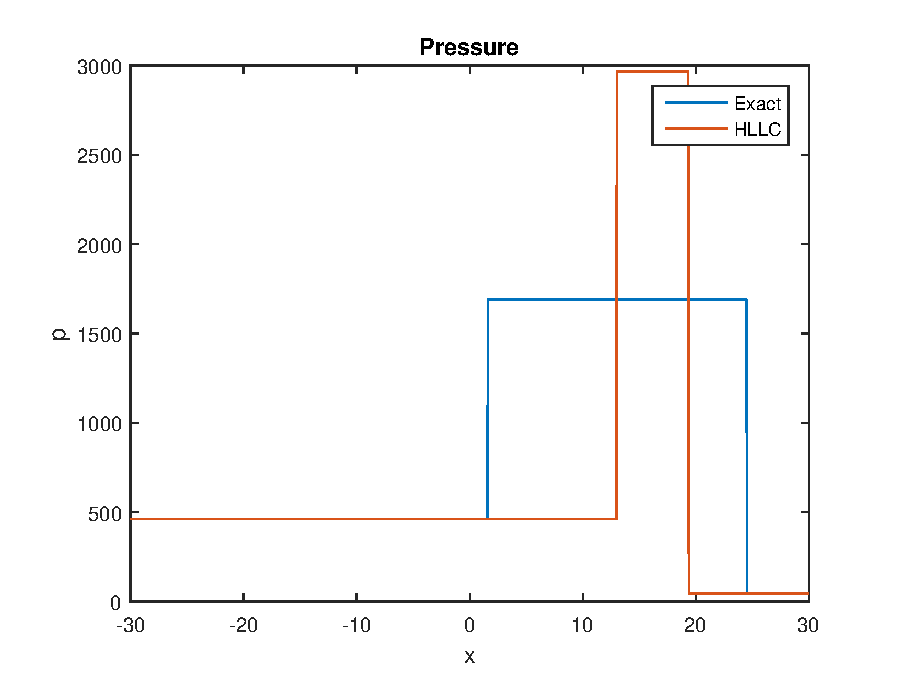
\includegraphics[width=3in]{dubShockP}
\caption{Exact solution of the 2D euler equations with initial conditions (56). Solution evolved until $t=2$ with ideal gas constant $\gamma=1.4$.}
\end{figure}

\textbf{Case 2. Double Rarefaction}
\bq \mbf{W}_L=\left[\begin{array}{c}1\\ -2\\ -3\\ .4\end{array}\right],\;\;\; \mbf{W}_R=\left[\begin{array}{c}1\\2\\3\\.4\end{array}\right].\eq
The exact solution is printed in figure 6. We see there that the change in the tangential velocity jumps only at the contact located at $x=0,$ even as the density remains constant in that field.\\

\begin{figure}[ht]
\centering
\includegraphics[width=3in]{dubRareDen}
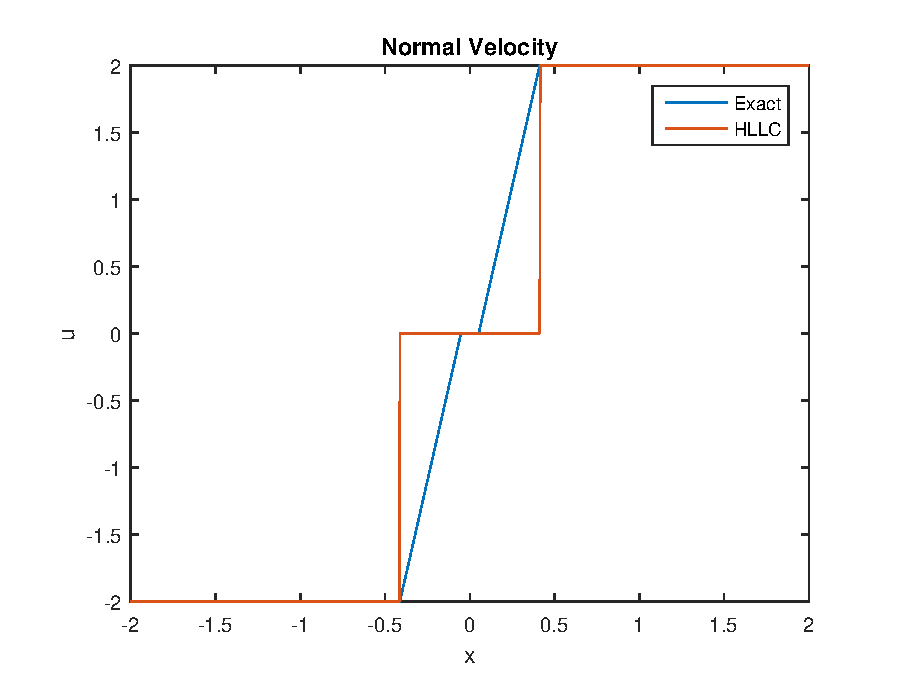
\includegraphics[width=3in]{dubRareU}\\
\includegraphics[width=3in]{dubRareV}
\includegraphics[width=3in]{dubRareP}
\caption{Exact solution of the 2D euler equations with initial conditions (57). Solution evolved until $t=.15$ with ideal gas constant $\gamma=1.4$.}
\end{figure}
\textbf{Case 3. Shocktube}
\bq \mbf{W}_L=\left[\begin{array}{c}1\\ 0\\ 1\\ 1\end{array}\right],\;\;\; \mbf{W}_R=\left[\begin{array}{c}1.5\\0\\0\\2\end{array}\right].\eq
The exact solution is then located in figure 7. In figure 7, we can see the left shock and right rarefaction, along with a well resolved contact discontinuity around $x=-0.2$
\begin{figure}[h]
\centering
\includegraphics[width=2.5in]{tubeDen}
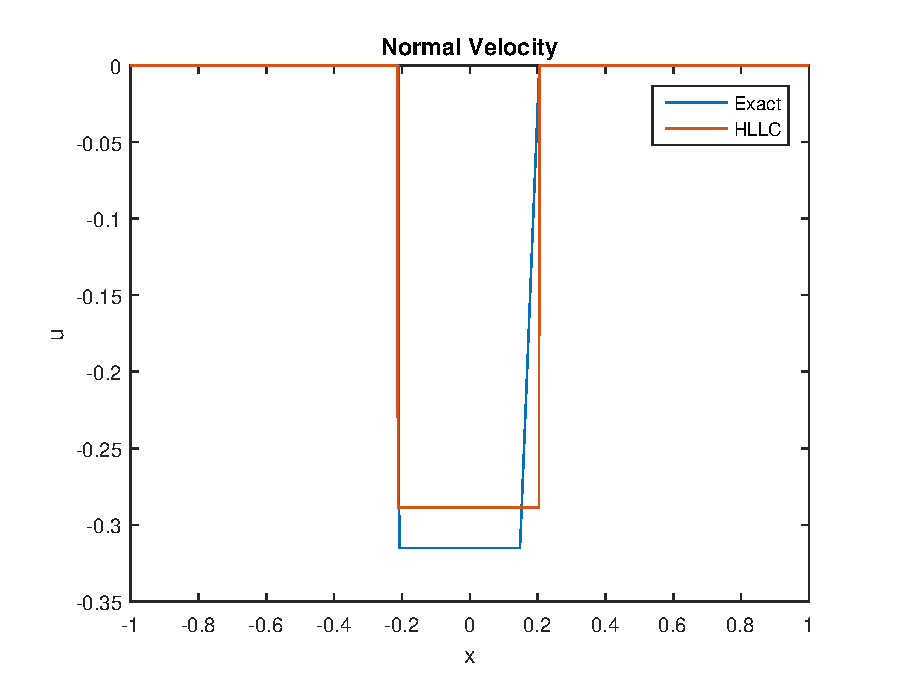
\includegraphics[width=2.5in]{tubeU}\\
\includegraphics[width=2.5in]{tubeV}
\includegraphics[width=2.5in]{tubeP}
\caption{Exact solution of the 2D euler equations with initial conditions (58). Solution evolved until $t=.15$ with ideal gas constant $\gamma=1.4.$}
\end{figure}
\end{subsection}
\begin{subsection}{Numerical Convergence Results}
As the two Cartesian solvers can be run with the same initial data (just choosing x=r and y=s) on a unit square grid, the convergence question really only boils down to the order of the flux calculations, since the time step is second order accurate. Unfortunately, since my boundary conditions are non-physical I can only demonstrate 1/2 order convergence in either case. Neither Richardson extrapolation nor the manufactured solution method have proven successful in showing convergence of any kind, likely due to a combination of choosing poor initial conditions/exact solutions and the nonphysical boundary conditions.\\
To show 1/2 order convergence, I ran the numerical solver with 2 vertical grid points and $M$ horizontal grid points with Riemann initial data using both the HLLC solver and the exact solver to determine intercell fluxes, and compared the solution to the exact solution. I was unable to successfully implement the Roe solver in time (it's close!). The convergence results are located in figure 8. 
\begin{figure}[hb]
\centering
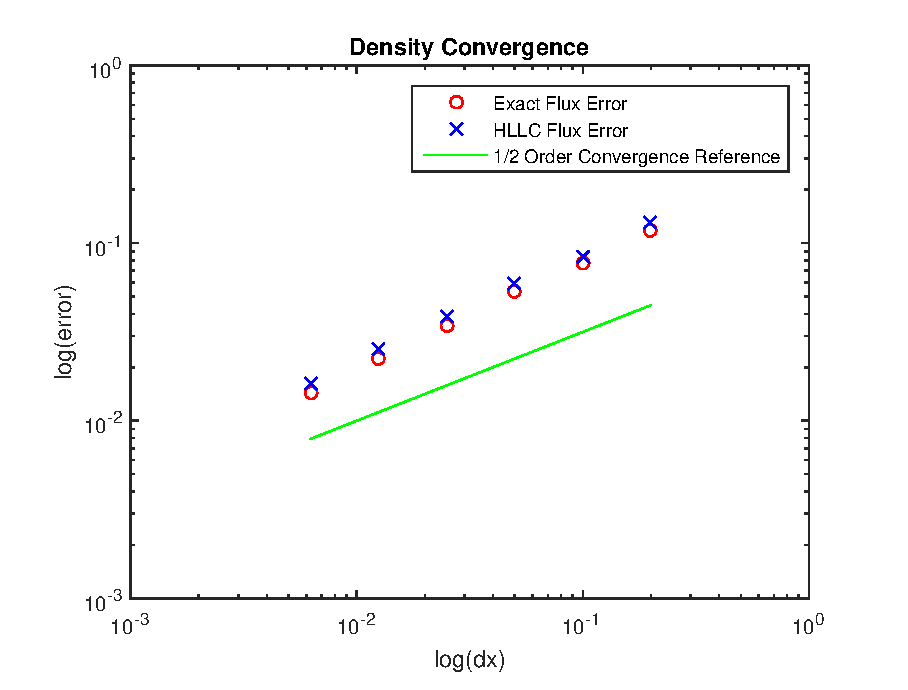
\includegraphics[width=2.5in]{eulerconv1}
\includegraphics[width=2.5in]{eulerconv2}
\caption{Logarithmic plot of the convergence rate of numerical solution methods given Riemann initial data(left) and smooth initial data (right)}
\end{figure}
Although the convergence results printed in figure 8 for smooth data shows divergence, the error is still small even for 6400 grid points. The smooth data is from the twilight zone method, which we looked at together. The issue remains unfixed.
\end{subsection}
\end{section}

\begin{section}{Conclusion}
In this paper we have outlined 3 intercell flux calculators - an adaptive iterative exact solver, an HLLC approximate solver and a Roe approximate solver, along with three discretizations for certain choices of domains and computational grids. We have presented some convergence results, but certainly not enough to justify any discretization included in the paper. More time is certainly necessary to look at these things again in a different light.\\
Future directions for improvement upon this work include showing convergence, implementing physical boundary conditions, automating grid generation techniques for both non-Cartesian domain solvers, implementing high-order methods and generalizing to the full 3D equations.
\end{section}

\iffalse

\fi
\newpage
\appendix
\section{Code Appendix}
Exact Riemann Euler Equation Solver
\begin{lstlisting}
function [w]=exactEuler2D(wL,wR,gamma,x,t,Qtol)
%exactEuler2D solves the Riemann problem exact for the 2D
%Euler equations in primitive variables with ideal gas
%constituive law
%   Input:
%       wL=left initial data
%       wR=right initial data
%       gamma=ideal gas constant
%       x=domain
%       t=time
%       Qtol=user specified tolerance
%   Output:
%       w=solution at time t

%% Define primitive variable initial states
rhoL=wL(1);
rhoR=wR(1);
tvL=wL(2);
tvR=wR(2);
nvL=wL(3);
nvR=wR(3);
pL=wL(4);
pR=wR(4);

%Sound Speeds
if pL/rhoL<0
    fprintf('Imaginary Sound Speed\n');
    fprintf('p_l=%d,rho_l=%d\n',pL,rhoL);
    return
elseif  pR/rhoR<0
    fprintf('Imaginary Sound Speed\n');
    fprintf('p_r=%d,rho_r=%d\n',pR,rhoR)
    return
end
cL=sqrt(gamma*pL/rhoL);
cR=sqrt(gamma*pR/rhoR);

%Check Pressure positivity:
if 2*(cL+cR)/(gamma-1)<(tvR-tvL)
    fprintf('Vacuum is generated by data\n');
    return
end

%% Initial Guess
lmax=10;
tol=1e-6;
%Linearized Guess
p0Lin=.5*(pL+pR)-(tvR-tvL)*(rhoL+rhoR)*(cL+cR)/8;
p0Lin=max([p0Lin,tol]);
%Double Rarefaction guess:
pRare=((cL+cR-.5*(gamma-1)*(tvR-tvL))/(cL/pL^((gamma-1)/...
    (2*gamma))+cR/pR^((gamma-1)/(2*gamma))))^(2*gamma/(gamma-1));
%Double Shock guess:
gL=(2/((gamma+1)*rhoL)/(p0Lin+(gamma-1)/(gamma+1)*pL))^.5;
gR=(2/((gamma+1)*rhoR)/(p0Lin+(gamma-1)/(gamma+1)*pR))^.5;

p0Shock=(pL*gL+pR*gR-(tvR-tvL))/(gL+gR);
p0Shock=max([p0Shock,tol]);
% Determine Best Initial guess:
pmax=max([pRare,p0Shock,p0Lin]);
pmin=min([pRare,p0Shock,p0Lin]);
Q=pmax/pmin;
pStar=p0Lin;
if Q<Qtol && pmin<pStar&& pStar<pmax
    p=p0Lin;
else if pStar<=pmin
        p=pRare;
    else
        p=p0Shock;
    end
end

%% Newton Iteration to find middle (star) state:

for l=1:lmax
    [lwave,locusL,derivL]=fk(p,pL,rhoL,gamma);
    [rwave,locusR,derivR]=fk(p,pR,rhoR,gamma);
    pNew=p-(locusL+locusR+tvR-tvL)/(derivL+derivR);
    CHA=2*abs((pNew-p)/(pNew+p));
    p=pNew;
    if CHA<Qtol
        fprintf('Newton Iteration Converged with %f iterations \n', l);
        break
    end
end

%% Construct rest of primitive variables and sound speeds:
pM = p;
[rhoML,rhoMR]=rhofinder(rhoL,rhoR,pM,pL,pR,gamma,lwave,rwave);
tvM= .5*(tvL+tvR)+.5*(locusR-locusL);
cML=sqrt(gamma*pM/rhoML);
cMR=sqrt(gamma*pM/rhoMR);
%% Construct Solution
w=zeros(4,numel(x));
for j=1:numel(x);
    S=x(j)/t;
if S<tvM
    %left
    if pL<pM
        %Shock
        Sl=tvL-cL*((gamma+1)/...
            (2*gamma)*pM/pL+(gamma-1)/(2*gamma))^.5;
        if S<Sl
            w(:,j)=[rhoL;tvL;nvL;pL];
        else
            w(:,j)=[rhoML;tvM;nvL;pM];
        end
    else
        %Rarefaction
        Shl=tvL-cL;
        Stl=tvM-cML;
        if S<Shl
            w(:,j)=[rhoL;tvL;nvL;pL];
        elseif S>Stl
            w(:,j)=[rhoML;tvM;nvL;pM];
        else
            [rho,v,p]=rareleft(rhoL,tvL,pL,cL,gamma,S);
            w(:,j)=[rho;v;nvL;p];
        end
    end
else
    if pR<pM
        %Shock
        Sr=tvR+cR*((gamma+1)/...
            (2*gamma)*pM/pR+(gamma-1)/(2*gamma))^.5;
        if S>Sr
            w(:,j)=[rhoR;tvR;nvR;pR];
        else
            w(:,j)=[rhoMR;tvM;nvR;pM];
        end
    else
        %Rarefaction
        Shr=tvR+cR;
        Str=tvM+cMR;
        if S>Shr
            w(:,j)=[rhoR;tvR;nvR;pR];
        elseif S<Str
            w(:,j)=[rhoMR;tvM;nvR;pM];
        else
            [rho,v,p]=rareright(rhoR,tvR,pR,cR,gamma,S);
            w(:,j)=[rho;v;nvR;p];
        end
    end
end
end


%% Auxillary Functions for Riemann solver
%Determines expressions for the newton iteration
    function [kWave,locusK,derivK]=fk(p,pK,rhoK,gamma)
        if pK>=p %Rarefaction
            locusK=2*sqrt(gamma*pK/rhoK)/(gamma-1)*...
                ((p/pK)^((gamma-1)/(2*gamma))-1);
            derivK=((p/pK)^((gamma-1)/(2*gamma))...
                *sqrt(gamma*pK/rhoK))/(p*gamma);
            kWave=0;
        else %Shock
            locusK=(p-pK)*(2/((gamma+1)*rhoK)/...
                (p+(gamma-1)/(gamma+1)*pK))^.5;
            derivK=sqrt(1/(2*rhoK))*(p*(1+gamma)+pK*(3*gamma-1))...
                /((p*(1+gamma)+pK*(gamma-1))^1.5);
            kWave=1;
        end
    end

%Finds middle rho states
    function [rhoML,rhoMR]=rhofinder(rhoL,rhoR,p,pL,pR,gamma,lWave,rWave)
        if lWave==0
            rhoML=rhoL*(p/pL)^(1/gamma);
            if rWave==0
                rhoMR=rhoR*(p/pR)^(1/gamma);
            else
                rhoMR=rhoR*(p/pR+(gamma-1)/(gamma+1))/...
                    ((gamma-1)/(gamma+1)*(p/pR)+1);
            end
        else
            rhoML=rhoL*(p/pL+(gamma-1)/(gamma+1))/...
                ((gamma-1)/(gamma+1)*(p/pL)+1);
            if rWave==0
                rhoMR=rhoR*(p/pR)^(1/gamma);
            else
                rhoMR=rhoR*(p/pR+(gamma-1)/(gamma+1))/...
                    ((gamma-1)/(gamma+1)*(p/pR)+1);
            end
        end
    end
% Defines solution in left rarefaction
    function [rho,v,p]=rareleft(rhoL,tvL,pL,cL,gamma,S)
        rho=rhoL*(2/(gamma+1)+(gamma-1)/((gamma+1)*cL)...
            *(tvL-S))^(2/(gamma-1));
        v=2/(gamma+1)*(cL+(gamma-1)/2*tvL+S);
        p=pL*(2/(gamma+1)+(gamma-1)/((gamma+1)*cL)...
            *(tvL-S))^(2*gamma/(gamma-1));
    end
%Defines solution in right rarefaction
    function [rho,v,p]=rareright(rhoR,tvR,pR,cR,gamma,S)
        rho=rhoR*(2/(gamma+1)-(gamma-1)/((gamma+1)*cR)...
            *(tvR-S))^(2/(gamma-1));
        v=2/(gamma+1)*(-cR+(gamma-1)/2*tvR+S);
        p=pR*(2/(gamma+1)-(gamma-1)/((gamma+1)*cR)...
            *(tvR-S))^(2*gamma/(gamma-1));
    end

end

\end{lstlisting}
HLLC Rieman Euler Equation Solver
\begin{lstlisting}
function [u]=HLLCEuler2D(wL,wR,gamma,x,t)
%define nice variable names
rhoL=wL(1);
rhoR=wR(1);
tvL=wL(2);
tvR=wR(2);
nvL=wL(3);
nvR=wR(3);
pL=wL(4);
pR=wR(4);
aL=sqrt(gamma*pL/rhoL);
aR=sqrt(gamma*pR/rhoR);
EL=.5*rhoL*(tvL^2+nvL^2)+pL/(gamma-1);
ER=.5*rhoR*(tvR^2+nvR^2)+pR/(gamma-1);
uL=[rhoL;rhoL*tvL;rhoL*nvL;EL];
uR=[rhoR;rhoR*tvR;rhoR*nvR;ER];

%Compute Pressure Estimate
rhob=.5*(rhoL+rhoR);
ab=.5*(aL+aR);
ppvrs=.5*(pL+pR)-.5*(tvR-tvL)*rhob*ab;
pS=max(0,ppvrs);

%Compute Wave Speed Estimates
qL=findq(pS,pL,gamma);
qR=findq(pS,pR,gamma);
SL=tvL-aL*qL;
SR=tvR+aR*qR;

SS=(pR-pL+rhoL*tvL*(SL-tvL)-rhoR*tvR*(SR-tvR))/...
    (rhoL*(SL-tvL)-rhoR*(SR-tvR));

%Construct Solution
u=zeros(4,numel(x));
for i=1:numel(x)
    xi=x(i)/t;
    if xi<SL
        u(:,i)=uL;
    elseif SL<=xi && xi<= SS
        u(:,i)=rhoL*(SL-tvL)/(SL-SS)*[1;SS;nvL;...
            EL/rhoL+(SS-tvL)*(SS+pL/(rhoL*(SL-tvL)))];
    elseif SS<= xi && xi<= SR
        u(:,i)=rhoR*(SR-tvR)/(SR-SS)*[1;SS;nvR;...
            ER/rhoR+(SS-tvR)*(SS+pR/(rhoR*(SR-tvR)))];
    elseif xi>=SR
        u(:,i)=uR;
    end
end
end

function qK=findq(pS,pK,gamma)
if pS<=pK
    qK=1;
else
    qK=sqrt(1+(gamma+1)/(2*gamma)*(pS/pK-1));
end
end

\end{lstlisting}
2D Numerical Euler Equation Solver
\begin{lstlisting}
function [data]=numEuler2D(cuInit,gamma,dx,dy,cfl,tF,Case,Order,iBound)
%numEuler2D solves the 2D Euler equations, with ideal gas
%constitutive law, numerically given some initial data
%   Inputs:
%       uInit=4xM matrix of initial data
%       gamma=ideal gas constant
%       cfl=cfl number
%       tF=final time
%       Case=type of numerical method
%       Order=Order of numerical method
%   Outputs:
%       data=primitive data saved at requested snapshot times
%       time=time(s) at which data was saved

%% Initialize Variables

%Give large bound on time for loop to end
dtMax=1e-1;
dtMin=1e-6;
nMax=tF/dtMin;

% Find total number of grid points including ghost cells
M=size(cuInit,1);
N=size(cuInit,2);

ng=Order;
Mtot=M+2*ng;
Ntot=N+2*ng;
ja=ng+1;
jb=Mtot-1;
ka=ng+1;
kb=Ntot-1;

%Initialize vectors
data=zeros(M,N,4);
xFluxMat=zeros(Mtot-1,N,4);
yFluxMat=zeros(M,Ntot-1,4);
timeNow=0;
cu=zeros(Mtot,Ntot,4);

%% Set Initial Conditions
cu(ja:jb,ka:kb,:)=cuInit;
%Set BCs on initial conditions
[cu]=setBCs(cu,ja,jb,ka,kb,Order,iBound);
%Calculate initial dt
[prim]=convertVar(cu,gamma,Mtot,Ntot);
xLamMax=1e-6;
yLamMax=1e-6;
for j=(ja-1):jb
    for k=(ka-1):kb
        [~,xLam]=xnumFlux(Case,prim(j,k,:),...
            prim(j+1,k,:),gamma);
        [~,yLam]=ynumFlux(Case,prim(j,k,:),...
            prim(j,k+1,:),gamma);
        if abs(xLam)>xLamMax
            xLamMax=abs(xLam);
        end
        if abs(yLam)>yLamMax
            yLamMax=abs(yLam);
        end
    end
end
%% Main Loop
for n=1:nMax
    %Convert conserved variables to primitive variables
    [prim]=convertVar(cu,gamma,Mtot,Ntot);
    
    %set dt
    dt=dtMax;
    dt=min(dt,cfl*dx*dy/(xLamMax*dy+yLamMax*dx));
    %Adjust time step to end at tF
    if timeNow+dt>tF
        dt=tF-timeNow;
    end
    %Compute Fluxes
    xLamMax=1e-6;
    yLamMax=1e-6;
    for j=(ja-1):jb
        for k=(ka-1):kb
            [fluxOut,xLam]=xnumFlux(Case,prim(j,k,:),...
                prim(j+1,k,:),gamma);
            xFluxMat(j,k,:)=fluxOut;
            [fluxOut,yLam]=ynumFlux(Case,prim(j,k,:),...
                prim(j,k+1,:),gamma);
                yFluxMat(j,k,:)=fluxOut;
            if abs(xLam)>xLamMax
                xLamMax=abs(xLam);
            end
            if abs(yLam)>yLamMax
                yLamMax=abs(yLam);
            end
        end
    end
    %Update Solution
    for j=ja:jb
        for k=ka:kb
            cu(j,k,:)=cu(j,k,:)-...
                (dt/dx)*(xFluxMat(j,k,:)-xFluxMat(j-1,k,:))-...
                (dt/dy)*(yFluxMat(j,k,:)-yFluxMat(j,k-1,:));
        end
    end
    
    %Set BCs
    cu=setBCs(cu,ja,jb,ka,kb,Order,iBound);
    
    %Calculate time
    timeNow=timeNow+dt;
    %Check if run has completed and save solution
    if timeNow>tF-eps
        data=cu(ja:jb,ka:kb,:);
        break
    end
end
%% Auxillary Functions

%% Bounday Conditions
    function [u]=setBCs(u,ja,jb,ka,kb,Order,iBound)
        if Order==1
            if iBound==1 %Transmissive everywhere
                for k=ka:kb %#ok<*FXUP>
                    u(ja-1,k,:)=u(ja+1,k,:);
                    u(jb+1,k,:)=u(jb-1,k,:);
                end
                for j=ja:jb
                    u(j,ka-1,:)=u(j,ka+1,:);
                    u(j,kb+1,:)=u(j,kb-1,:);
                end
            elseif iBound==2 %Reflective everywhere
                for k=ka:kb
                    u(ja-1,k,:)=u(ja,k,:);
                    u(ja-1,k,2)=-u(ja,k,2);
                    u(jb+1,k,:)=u(jb-1,k,:);
                    u(jb+1,k,2)=-u(jb-1,k,:);
                end
                for j=ja:jb
                    u(j,ka-1,:)=u(j,ka,:);
                    u(j,ka-1,2)=-u(j,ka,2);
                    u(j,kb+1,:)=u(j,kb,:);
                    u(j,kb+1,2)=-u(j,kb,2);
                end
            elseif iBound==3 %Transmissive horiz,
                %Reflective vert
                for k=ka:kb %#ok<*FXUP>
                    u(ja-1,k,:)=u(ja+1,k,:);
                    u(jb+1,k,:)=u(jb-1,k,:);
                end
                for j=ja:jb
                    u(j,ka-1,:)=u(j,ka,:);
                    u(j,ka-1,2)=-u(j,ka,2);
                    u(j,kb+1,:)=u(j,kb,:);
                    u(j,kb+1,2)=-u(j,kb,2);
                end
            elseif iBound==4 %Reflective left,top,
                %Transmissive bot,right
                for k=ka:kb
                    u(ja-1,k,:)=u(ja,k,:);
                    u(ja-1,k,2)=-u(ja,k,2);
                    u(jb+1,k,:)=u(jb-1,k,:);
                end
                for j=ja:jb
                    u(j,ka-1,:)=u(j,ka+1,:);
                    u(j,kb+1,:)=u(j,kb,:);
                    u(j,kb+1,2)=-u(j,kb,2);
                end
            elseif iBound==5 %Reflective left
                %Transmissive else
                for k=ka:kb
                    u(ja-1,k,:)=u(ja,k,:);
                    u(ja-1,k,2)=-u(ja,k,2);
                    u(jb+1,k,:)=u(jb-1,k,:);
                end
                for j=ja:jb
                    u(j,ka-1,:)=u(j,ka+1,:);
                    u(j,kb+1,:)=u(j,kb-1,:);
                end
                
            elseif iBound==6 %Transmissive left
                %Reflective else
                for k=ka:kb
                    u(ja-1,k,:)=u(ja+1,k,:);
                    u(jb+1,k,:)=u(jb-1,k,:);
                    u(jb+1,k,2)=-u(jb-1,k,:);
                end
                for j=ja:jb
                    u(j,ka-1,:)=u(j,ka,:);
                    u(j,ka-1,2)=-u(j,ka,2);
                    u(j,kb+1,:)=u(j,kb,:);
                    u(j,kb+1,2)=-u(j,kb,2);
                end
            end
        end
    end

%% Primitive Variable Converter
    function [w]=convertVar(u,gamma,Mtot,Ntot)
        %density
        rho=u(:,:,1);
        %momenta
        mx=u(:,:,2);
        my=u(:,:,3);
        %energy
        E=u(:,:,4);
        w(:,:,1)=rho;
        for i=1:Mtot
            for j=1:Ntot
                %Velocities
                w(i,j,2)=mx(i,j)/rho(i,j);
                w(i,j,3)=my(i,j)/rho(i,j);
                %Pressure
                w(i,j,4)=(gamma-1)*(E(i,j)-...
                    .5*(mx(i,j)^2+my(i,j)^2)/rho(i,j));
            end
        end
    end

%% Numerical Flux Functions
    function [fluxOut,xLam]=xnumFlux(Case,A,B,gamma)
	  if Case==1
            %Exact
            [z,xLam]=eulerExact(A,B,gamma,1e-8);
            fluxOut=xFlux(z,gamma);
        elseif Case==2
            %HLLC
            [fluxOut,xLam]=eulerHLLC(A,B,gamma);
        end
    end
    function [fluxOut,yLam]=ynumFlux(Case,A,B,gamma)
        
        C(:,:,1)=A(:,:,1);
        C(:,:,2)=A(:,:,3);
        C(:,:,3)=A(:,:,2);
        C(:,:,4)=A(:,:,4);
        D(:,:,1)=B(:,:,1);
        D(:,:,2)=B(:,:,3);
        D(:,:,3)=B(:,:,2);
        D(:,:,4)=B(:,:,4);
        if Case==1
            [z,yLam]=eulerExact(C,D,gamma,1e-8);
            q=z;
            q(2)=z(3);
            q(3)=z(2);
            fluxOut=yFlux(q,gamma);
            
        elseif Case==2
            [z,yLam]=eulerHLLC(C,D,gamma);
            fluxOut=z;
            fluxOut(2)=z(3);
            fluxOut(3)=z(2);
        end
    end

%% Flux Calculators
    function z=xFlux(A,gamma)
        rho=A(1);
        u=A(2);
        v=A(3);
        p=A(4);
        E=p/(gamma-1)+.5*rho*(u^2+v^2);
        z=[rho*u;rho*u^2+p;rho*u*v;u*(E+p)];
    end
    function z=yFlux(A,gamma)
        rho=A(1);
        u=A(2);
        v=A(3);
        p=A(4);
        E=p/(gamma-1)+.5*rho*(u^2+v^2);
        z=[rho*v;rho*u*v;rho*v^2+p;v*(E+p)];
    end
    
    %% HLLC Approximate Riemann Solver
    function [fluxOut,lam]=eulerHLLC(wL,wR,gamma)
        rhoL=wL(1);
        rhoR=wR(1);
        tvL=wL(2);
        tvR=wR(2);
        nvL=wL(3);
        nvR=wR(3);
        pL=wL(4);
        pR=wR(4);
        aL=sqrt(gamma*rhoL/pL);
        aR=sqrt(gamma*rhoR/pR);
        EL=.5*rhoL*(tvL^2+nvL^2)+pL/(gamma-1);
        ER=.5*rhoR*(tvR^2+nvR^2)+pR/(gamma-1);
        uL=[rhoL;rhoL*tvL;rhoL*nvL;EL];
        uR=[rhoR;rhoR*tvR;rhoR*nvR;ER];
        
        rhob=.5*(rhoL+rhoR);
        ab=.5*(aL+aR);
        ppvrs=.5*(pL+pR)-.5*(tvR-tvL)*rhob*ab;
        ps=max(0,ppvrs);
        qL=qFind(ps,pL,gamma);
        qR=qFind(ps,pR,gamma);
        SL=tvL-aL*qL;
        SR=tvR+aR*qR;
        SS=(pR-pL+rhoL*tvL*(SL-tvL)-rhoR*tvR*(SR-tvR))/...
            (rhoL*(SL-tvL)-rhoR*(SR-tvR));
        if 0 <= SL
            lam=abs(tvL)+aL;
            fluxOut=xFlux(wL,gamma);
        elseif SL<=0 && 0<=SS
            lam=abs(tvL)+aL;
            uSL=rhoL*(SL-tvL)/(SL-SS)*[1;SS;nvL;...
                EL/rhoL+(SS-tvL)*(SS+pL/(rhoL*(SL-tvL)))];
            FL=xFlux(wL,gamma);
            fluxOut=FL+SL*(uSL-uL);
        elseif SS<=0 && 0<=SR
            lam=abs(tvR)+aR;
            uSR=rhoR*(SR-tvR)/(SR-SS)*[1;SS;nvR;...
                ER/rhoR+(SS-tvR)*(SS+pR/(rhoR*(SR-tvR)))];
            FR=xFlux(wR,gamma);
            fluxOut=FR+SR*(uSR-uR);
        elseif 0>=SR
            lam=abs(tvR)+aR;
            fluxOut=xFlux(wR,gamma);
        end
        
    end

%% HLLC Aux Functions
    function q=qFind(pS,pK,gamma)
        if pS<=pK
            q=1;
        else
            q=sqrt(1+(gamma+1)/(2*gamma)*(pS/pK-1));
        end
    end


%% Exact Riemann Solver
    function [w,lam]=eulerExact(wL,wR,gamma,Qtol)
        %exactEuler2D solves the Riemann problem exact for the 2D
        %Euler equations in primitive variables with ideal gas
        %constituive law
        %   Input:
        %       wL=left initial data
        %       wR=right initial data
        %       gamma=ideal gas constant
        %       x=domain
        %       t=time
        %       Qtol=user specified tolerance
        %   Output:
        %       w=solution at time t
        
        %% Define primitive variable initial states
        rhoL=wL(1);
        rhoR=wR(1);
        tvL=wL(2);
        tvR=wR(2);
        nvL=wL(3);
        nvR=wR(3);
        pL=wL(4);
        pR=wR(4);
        
        %Sound Speeds
        if pL/rhoL<0
            fprintf('Imaginary Sound Speed\n');
            fprintf('p_l=%d,rho_l=%d\n',pL,rhoL);
            return
        elseif  pR/rhoR<0
            fprintf('Imaginary Sound Speed\n');
            fprintf('p_r=%d,rho_r=%d\n',pR,rhoR)
            return
        end
        cL=sqrt(gamma*pL/rhoL);
        cR=sqrt(gamma*pR/rhoR);
        
        %Check Pressure positivity:
        if 2*(cL+cR)/(gamma-1)<(tvR-tvL)
            fprintf('Vacuum is generated by data\n');
            return
        end
        
        %% Initial Guess
        lmax=10;
        tol=1e-6;
        %Linearized Guess
        p0Lin=.5*(pL+pR)-(tvR-tvL)*(rhoL+rhoR)*(cL+cR)/8;
        p0Lin=max([p0Lin,tol]);
        %Double Rarefaction guess:
        pRare=((cL+cR-.5*(gamma-1)*(tvR-tvL))/(cL/pL^((gamma-1)/(2*gamma))+...
            cR/pR^((gamma-1)/(2*gamma))))^(2*gamma/(gamma-1));
        %Double Shock guess:
        gL=(2/((gamma+1)*rhoL)/(p0Lin+(gamma-1)/(gamma+1)*pL))^.5;
        gR=(2/((gamma+1)*rhoR)/(p0Lin+(gamma-1)/(gamma+1)*pR))^.5;
        
        p0Shock=(pL*gL+pR*gR-(tvR-tvL))/(gL+gR);
        p0Shock=max([p0Shock,tol]);
        % Determine Best Initial guess:
        pmax=max([pRare,p0Shock,p0Lin]);
        pmin=min([pRare,p0Shock,p0Lin]);
        Q=pmax/pmin;
        pStar=p0Lin;
        if Q<Qtol && pmin<pStar&& pStar<pmax
            p=p0Lin;
        else if pStar<pmin
                p=pRare;
            else
                p=p0Shock;
            end
        end
        
        %% Newton Iteration to find middle (star) state:
        
        for l=1:lmax
            [lwave,locusL,derivL]=fk(p,pL,rhoL,gamma);
            [rwave,locusR,derivR]=fk(p,pR,rhoR,gamma);
            pNew=p-(locusL+locusR+tvR-tvL)/(derivL+derivR);
            CHA=2*abs((pNew-p)/(pNew+p));
            p=pNew;
            if CHA<Qtol
                %fprintf('Newton Iteration Converged with %f iterations \n', n);
                break
            end
        end
        
        %% Construct rest of primitive variables and sound speeds:
        pM = p;
        [rhoML,rhoMR]=rhofinder(rhoL,rhoR,pM,pL,pR,gamma,lwave,rwave);
        tvM= .5*(tvL+tvR)+.5*(locusR-locusL);
        cML=sqrt(gamma*pM/rhoML);
        cMR=sqrt(gamma*pM/rhoMR);
        %% Construct Solution
        S=0;
        if S<tvM
            %left
            if pL<pM
                %Shock
                Sl=tvL-cL*((gamma+1)/...
                    (2*gamma)*pM/pL+(gamma-1)/(2*gamma))^.5;
                if S<Sl
                    w=[rhoL;tvL;nvL;pL];
                    lam=abs(tvL)+cL;
                else
                    w=[rhoML;tvM;nvL;pM];
                    lam=abs(tvM)+cML;
                end
            else
                %Rarefaction
                Shl=tvL-cL;
                Stl=tvM-cML;
                if S<Shl
                    w=[rhoL;tvL;nvL;pL];
                    lam=abs(tvL)+cL;
                elseif S>Stl
                    w=[rhoML;tvM;nvL;pM];
                    lam=abs(tvM)+cML;
                else
                    [rho,v,p]=rareleft(rhoL,tvL,pL,cL,gamma,S);
                    w=[rho;v;nvL;p];
                    lam=abs(v)+sqrt(gamma*p/rho);
                end
            end
        else
            if pR<pM
                %Shock
                Sr=tvR+cR*((gamma+1)/...
                    (2*gamma)*pM/pR+(gamma-1)/(2*gamma))^.5;
                if S>Sr
                    w=[rhoR;tvR;nvR;pR];
                    lam=abs(tvR)+cR;
                else
                    w=[rhoMR;tvM;nvR;pM];
                    lam=abs(tvM)+cMR;
                end
            else
                %Rarefaction
                Shr=tvR+cR;
                Str=tvM+cMR;
                if S>Shr
                    w=[rhoR;tvR;nvR;pR];
                    lam=abs(tvR)+cR;
                elseif S<Str
                    w=[rhoMR;tvM;nvR;pM];
                    lam=abs(tvM)+cMR;
                else
                    [rho,v,p]=rareright(rhoR,tvR,pR,cR,gamma,S);
                    w=[rho;v;nvR;p];
                    lam=abs(v)+sqrt(gamma*p/rho);
                end
            end
        end
    end


%% Auxillary Functions for Riemann solver
%Determines expressions for the newton iteration
    function [kWave,locusK,derivK]=fk(p,pK,rhoK,gamma)
        if pK>=p %Rarefaction
            locusK=2*sqrt(gamma*pK/rhoK)/(gamma-1)*...
                ((p/pK)^((gamma-1)/(2*gamma))-1);
            derivK=((p/pK)^((gamma-1)/(2*gamma))...
                *sqrt(gamma*pK/rhoK))/(p*gamma);
            kWave=0;
        else %Shock
            locusK=(p-pK)*(2/((gamma+1)*rhoK)/...
                (p+(gamma-1)/(gamma+1)*pK))^.5;
            derivK=sqrt(1/(2*rhoK))*(p*(1+gamma)+pK*(3*gamma-1))...
                /((p*(1+gamma)+pK*(gamma-1))^1.5);
            kWave=1;
        end
    end

%Finds middle rho states
    function [rhoML,rhoMR]=rhofinder(rhoL,rhoR,p,pL,pR,gamma,lWave,rWave)
        if lWave==0
            rhoML=rhoL*(p/pL)^(1/gamma);
            if rWave==0
                rhoMR=rhoR*(p/pR)^(1/gamma);
            else
                rhoMR=rhoR*(p/pR+(gamma-1)/(gamma+1))/...
                    ((gamma-1)/(gamma+1)*(p/pR)+1);
            end
        else
            rhoML=rhoL*(p/pL+(gamma-1)/(gamma+1))/...
                ((gamma-1)/(gamma+1)*(p/pL)+1);
            if rWave==0
                rhoMR=rhoR*(p/pR)^(1/gamma);
            else
                rhoMR=rhoR*(p/pR+(gamma-1)/(gamma+1))/...
                    ((gamma-1)/(gamma+1)*(p/pR)+1);
            end
        end
    end
% Defines solution in left rarefaction
    function [rho,v,p]=rareleft(rhoL,tvL,pL,cL,gamma,S)
        rho=rhoL*(2/(gamma+1)+(gamma-1)/((gamma+1)*cL)...
            *(tvL-S))^(2/(gamma-1));
        v=2/(gamma+1)*(cL+(gamma-1)/2*tvL+S);
        p=pL*(2/(gamma+1)+(gamma-1)/((gamma+1)*cL)...
            *(tvL-S))^(2*gamma/(gamma-1));
    end
%Defines solution in right rarefaction
    function [rho,v,p]=rareright(rhoR,tvR,pR,cR,gamma,S)
        rho=rhoR*(2/(gamma+1)-(gamma-1)/((gamma+1)*cR)...
            *(tvR-S))^(2/(gamma-1));
        v=2/(gamma+1)*(-cR+(gamma-1)/2*tvR+S);
        p=pR*(2/(gamma+1)-(gamma-1)/((gamma+1)*cR)...
            *(tvR-S))^(2*gamma/(gamma-1));
    end

end
\end{lstlisting}

\end{document}